% Asset ID: AS2CorrelationAndRegressionLinesTikZ-001
% Source: CCEA AS2-DPI-LO005 + S1-Chp4-Correlation.pdf + teacher transcript
% Related section: Core Theory - Describing correlation
% Purpose: Show weak positive, weak negative, strong positive and no correlation.
\documentclass[tikz,border=6pt]{standalone}
\usepackage{amsmath}
\usetikzlibrary{arrows.meta}
\begin{document}
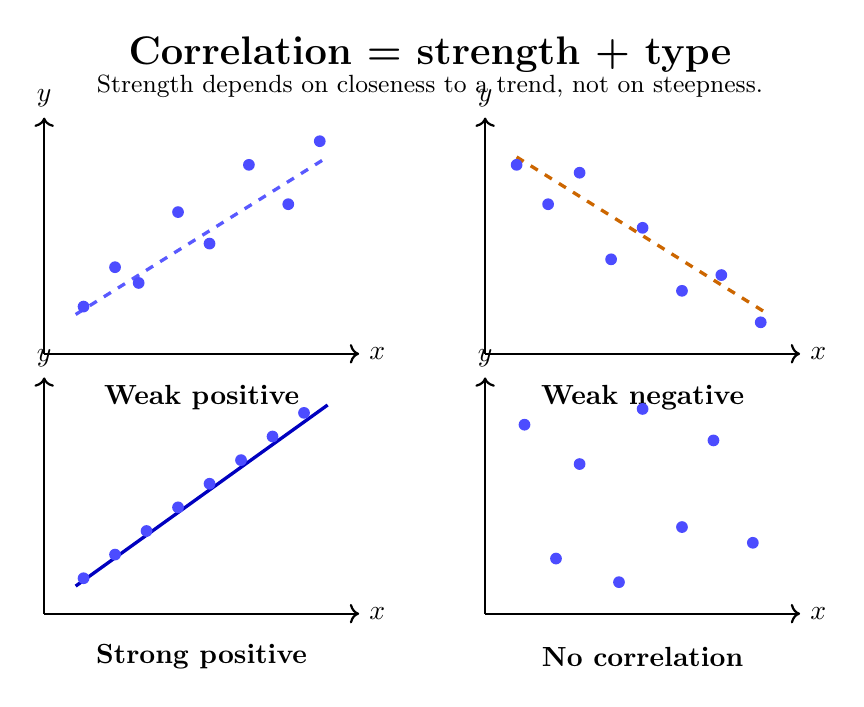
\begin{tikzpicture}[font=\sffamily,axis/.style={->, thick},trend/.style={very thick, dashed},point/.style={circle, fill=blue!70, inner sep=1.5pt}]
\newcommand{\miniAxes}{\draw[axis] (0,0) -- (4,0) node[right] {$x$};\draw[axis] (0,0) -- (0,3) node[above] {$y$};}
\node[font=\bfseries\Large] at (4.9,7.1) {Correlation = strength + type};
\node[font=\small] at (4.9,6.7) {Strength depends on closeness to a trend, not on steepness.};
\begin{scope}[shift={(0,3.3)}]\miniAxes\draw[trend, blue!65] (0.4,0.5) -- (3.6,2.5);\foreach \p in {(0.5,0.6),(0.9,1.1),(1.2,0.9),(1.7,1.8),(2.1,1.4),(2.6,2.4),(3.1,1.9),(3.5,2.7)}\node[point] at \p {};\node[font=\bfseries] at (2,-0.55) {Weak positive};\end{scope}
\begin{scope}[shift={(5.6,3.3)}]\miniAxes\draw[trend, orange!80!black] (0.4,2.5) -- (3.6,0.5);\foreach \p in {(0.4,2.4),(0.8,1.9),(1.2,2.3),(1.6,1.2),(2.0,1.6),(2.5,0.8),(3.0,1.0),(3.5,0.4)}\node[point] at \p {};\node[font=\bfseries] at (2,-0.55) {Weak negative};\end{scope}
\begin{scope}[shift={(0,0)}]\miniAxes\draw[very thick, blue!75!black] (0.4,0.35) -- (3.6,2.65);\foreach \p in {(0.5,0.45),(0.9,0.75),(1.3,1.05),(1.7,1.35),(2.1,1.65),(2.5,1.95),(2.9,2.25),(3.3,2.55)}\node[point] at \p {};\node[font=\bfseries] at (2,-0.55) {Strong positive};\end{scope}
\begin{scope}[shift={(5.6,0)}]\miniAxes\foreach \p in {(0.5,2.4),(0.9,0.7),(1.2,1.9),(1.7,0.4),(2.0,2.6),(2.5,1.1),(2.9,2.2),(3.4,0.9)}\node[point] at \p {};\node[font=\bfseries] at (2,-0.55) {No correlation};\end{scope}
\end{tikzpicture}
\end{document}
